%% This is file `dib-template.tex',
%%
%% Copyright 2020 Elsevier Ltd
%%
%% This file is part of the 'Elsarticle Bundle'.
%% ---------------------------------------------
%%
%% It may be distributed under the conditions of the LaTeX Project Public
%% License, either version 1.2 of this license or (at your option) any
%% later version.  The latest version of this license is in
%%    http://www.latex-project.org/lppl.txt
%% and version 1.2 or later is part of all distributions of LaTeX
%% version 1999/12/01 or later.
%%
%% The list of all files belonging to the 'Elsarticle Bundle' is
%% given in the file `manifest.txt'.
%%
%% Template article for Elsevier's document class `elsarticle'
%% with harvard style bibliographic references
%%
%% $Id: dib-template.tex 185 2020-08-07 09:06:08Z rishi $
%%
%% Use the option review to obtain double line spacing
%\documentclass[times,review,preprint]{elsarticle}

%% Use the options `final' to obtain the final layout
%% Use longtitle option to break abstract to multiple pages if overfull.
%% For Review pdf (With double line spacing)
%\documentclass[times,review]{elsarticle}
%% For abstracts longer than one page.
%\documentclass[times,review,longtitle]{elsarticle}
%% For Review pdf without preprint line
%\documentclass[times,review,nopreprintline]{elsarticle}
%% Final pdf
\documentclass[times,final]{elsarticle}
%%
%\documentclass[times,final,longtitle]{elsarticle}
%%

%%
%% Stylefile to load DIB template
\usepackage{dib}
\usepackage{framed,multirow}
\usepackage[linesnumbered,lined,boxed,commentsnumbered]{algorithm2e}
\usepackage{graphicx}

%% The amssymb package provides various useful mathematical symbols
\usepackage{amssymb}
\usepackage{latexsym}

%% For line numbers
%\usepackage[switch]{lineno}

% Following three lines are needed for this document.
% If you are not loading colors or url, then these are
% not required.
\usepackage{url}
\usepackage{xcolor}
\definecolor{newcolor}{rgb}{.8,.349,.1}

%%
\usepackage{longtable}
\usepackage[colorlinks]{hyperref}

\journal{Data in Brief}

\begin{document}

\verso{D. Rey Blanco \textit{et al.}}

\begin{frontmatter}

\dochead{Data Article}
%The article title must include the word 'data' or 'dataset'.
%Please avoid the use of acronyms and abbreviations where possible.
%For co-submission authors, the title should be unique,
%i.e. not the same as your research paper.
%A maximum of 250 characters is allowed.
\title{idealista18: A data package with real estate information in three major Spanish markets from the Idealista database }%
% \title{idealista18: A data package with real estate information in three major Spanish markets from the Idealista database \tnoteref{tnote1} }%
% \tnotetext[tnote1]{This is an example for title footnote coding.}
%Tip: here are a few examples of recent suitable article titles - these are short and clear:
%%Adolescent Rat Social Play: Amygdalar Proteomic and Transcriptomic Data
%%Execution Data Logs of a Supercomputer Workload Over its Extended Lifetime
%%Calgary Preschool Magnetic Resonance Imaging (MRI) Dataset]

%%Authors
\author[1]{David \snm{Rey Blanco}}
\author[1]{Pelayo \snm{González Arbues}}
% \author[1]{Pelayo \snm{González Arbues}\fnref{fn1}}
% \fntext[fn1]{This is author footnote for second author.}
\author[2]{Fernando \snm{López Hernández}}
\author[3]{Antonio \snm{Páez}\corref{cor1}}
%% Fourth author's email
\ead{paezha@mcmaster.ca}
\cortext[cor1]{Corresponding author:
  Tel.: +1-905-525-9140 ext 26099}

%%Affiliations
\address[1]{idealista, Plaza de las Cortes 5, 28014 Madrid, Spain}
\address[2]{Facultad de CC de la Empresa, C/ Real, 3. 30201 Cartagena, Murcia (Spain)}
\address[3]{School of Earth, Environment and Society, McMaster University, 1280 Main St W, Hamilton, Ontario L8S 4K1 Canada}

%\received{1 May 2013}
%\finalform{10 May 2013}
%\accepted{13 May 2013}
%\availableonline{15 May 2013}
%\communicated{S. Sarkar}


\begin{abstract}
%%%%
This dataset contains three items for each of the three major cities in Spain: Madrid, Barcelona and Valencia. The first data set contains real estate listings published on idealista portal in 2018. All listings have been enriched with cadastral information (i.e. building year of construction, built quality materials grade) plus some geographical features such as distance to relevant city areas and the coordinates themselves. To comply with european personal protection laws, we have processeed some sensitive variables yet preserving their spatial properties. The second data sets contains the neighborhood boundaries for each city, and third sets comprise a set of key points of interest for each municipality.
This dataset is suitable to house market analysis, hedonic house price models and other spatial research related with real estate markets.

\textbf{<falta cita/referencia al artículo>}

%\noindent[The Abstract should describe the data collection process, the analysis
%performed, the data, and their reuse potential. It should not provide
%conclusions or interpretive insights. If your article is being
%submitted via another Elsevier journal as a co-submission, please cite
%this research article in the abstract.

%\noindent\textbf{Tip:} do not use words such as
%`study', `results', and `conclusions' because a data article should be
%describing your data only.  Min 100 words - Max 500 words.]

%%%%
\end{abstract}

\begin{keyword}
%% Keywords
%[Include 4-8 keywords (or phrases) to facilitate others finding your
%article online.
%\noindent\textbf{Tip:} Try Google Scholar to find which terms are most common in your
%field. In biomedical fields, MeSH terms are a good 'common vocabulary'
%to draw from]
\KWD Property values\sep Spain\sep Spatial analysis\sep Machine learning\sep Hedonic price analysis
\end{keyword}

\end{frontmatter}

%% For linenumbers
%\linenumbers

{\fontsize{7.5pt}{9pt}\selectfont
%%%
\noindent\textbf{Specifications Table}

Every section of this table is mandatory.
Please enter information in the right-hand column and remove all the instructions
\begin{longtable}{|p{33mm}|p{94mm}|}
\hline
\endhead
\hline
\endfoot
Subject                & Geography, Economics\\
\hline
Specific subject area  & Spatial analysis, machine learning, hedonic price analysis\\
\hline
Type of data           & Tables\newline\\
%\clearpage
How data were acquired & multi-family listing records given by idealista portal \cite{idealista}\newline
                         Spanish central cadastral registry \cite{Catastro}\newline
                         Open street map \cite{OpenStreetMap}\newline
\\
\hline
Data format            & Spatially masked\\
\hline
Parameters for
data\newline
collection             & Data has been directly downloaded from the sources, cadastral and idealista data has been merged based on geographical location for each record
\\
% [Provide a brief description of which conditions were considered
%                          for data collection. Max 400 characters]

\hline
Description of
data\newline
collection             & idealista provided the complete record set \newline
                         cadastral information has been downloaded the open records published quarterly\newline
                         open street map has been downloaded from its open API
\\
\hline
Data source location   & Institution: Idealista\newline
                         City/Town/Region: Madrid, Barcelona, Valencia\newline
                         Country: Spain\newline
                         Latitude and longitude samples/data: EPSG:4326\newline
\\

%
%                          If you are describing secondary data, you are required to provide a list of
%                          the primary data sources used in the section.\newline
%
%                          Primary data sources:  ]\\
\hline
\hypertarget{target1}
{Data accessibility}   & Repository name: GitHub\newline
                         Direct URL to data: https://github.com/paezha/idealista18\newline
                         \\
\hline
Related
research\newline
article                & D. Rey Blanco, P. González Arbues, F. López Hernández, A. Páez, Using machine learning to identify spatial market segments: A reproducible study of major Spanish markets, Comput Environ Urban Syst. In Press.\newline
\end{longtable}
}
%%%

\section*{Value of the Data}

\begin{itemize}
\itemsep=0pt
\parsep=0pt
  \item A cleaned and enriched dataset consisting of real estate listings for three major cities in Spain. It has been constructed to analyze the impact of using machine learning models to identify spatial market segments when building house price hedonic models.
  \item The dataset can be used to extend the topic of automatic or semi-automatic identification of house market segments.
    \item The neighborhood boundaries combined with spatial patterns can be used to analyse the suitability of these boundaries as spatial dummy variables for real estate analyses purposes.
  \item The dataset can be enlarged with complementary spatial information to develop hedonic models.
  \item The data can be processed by quantitative analysis and statistical modeling to study the different factors that affect house prices in the three locations.
  \item Identification of spatial patterns in the real estate scope using the geo-referenced data points. For either value or urban patterns discovery.
\end{itemize}

\section*{Data Description}

\noindent
% [Individually describe each data file (i.e. figure 1, figure 2, table
% 1, dataset, raw data, supplementary data, etc.) that are included in
% this article. Please make sure you refer to every data file and provide
% a clear description for each - do not simply list them. No insight,
% interpretation, background or conclusions should be included in this
% section. Please include legends with any tables, figures or graphs.

This data package is composed of data objects corresponding to three major Spanish cities: quarterly single family listings, neighboorhood polygons and a set key of Points of Interest for each city. All spatial features, such as polygons and points, are expressed in geodetic coordinates using the \emph{EPSG:4326} coordinate reference system. The first block of data integrates properties published on idealista web site \cite{idealista}; each file contains the complete offering for a city for the four quarters in 2018. Idealista is the major real estate listing portal in Spain and also present in other southern european countries as Italy and Portugal. Each record contains the key found in listing ad\footnote{we will use the term \emph{ad} or \emph{listing} interchangeably to refer to a house published on the portal} plus a number of additional attribues from the Spanish cadastre \cite{Catastro}. The latter are described in the table \ref{table:data-assets-variables}, and the names for all these variables start with the prefix \emph{CAD}. Cadastral features asssignment is done by assigning the features of the nearest parcel to the coordinates \emph{LATITUDE} and \emph{LONGITUDE}. The measure scales for each variable has been defined according the theoretical framework proposed by \cite{stevens1946theory} that defines four scales: nominal, ordinal, interval and ratio.

\begin{footnotesize}
\begin{longtable}{p{40mm} c p{63mm}}
\caption{Description of the variables in the listing data set}\\
\label{table:data-assets-variables} \\
\hline
\hline
% \endhead
% \hline
% \endfoot
& &\\
\textbf{Variable} & \textbf{Mesurement scale} & \textbf{Description}\\
& &\\
\hline
ASSETID & Identifier & Unique identifier of the advertisement\\
PERIOD & Nominal (Date) & Expressed as YYYYMM, indicates the quarter when the ad was extracted. We used YYYY03 for the 1st quarter, YYYY06 the 2nd, YYYY09 for the 3rd and YYYY12 for the 4th\\
PRICE & Interval & Asking price for the ad at idealista expressed in euros\\
UNITPRICE & Interval & Asking price in euros per square meter (constructed area)\\
ADTYPOLOGYID & Nominal & Residential building type: multi-family: \emph{home}, single-familiy: \emph{chalet}\\
ADOPERATIONID & Nominal & Operation type for the ad: \emph{sale} or \emph{rent}\\
ROOMNUMBER & Ordinal & Number of bedrooms\\
BATHNUMBER & Ordinal & Number of bathrooms\\
HASTERRACE & Nominal & Dummy variable for terrace (takes 1 if there is a terrace, 0 otherwise\\
HASLIFT & Nominal & Dummy variable for lift (takes 1 if there is a lift in the building, 0 otherwise)\\
HASAIRCONDITIONING & Nominal & Dummy variable for AA (takes 1 if there is a AA, 0 otherwise)\\
AMENITYID & Nominal & Indicates the amenities included (1 - no furniture, no kitchen amenities, 2 - kitchen amenities, no furniture, 3 - kitchen amenities, furniture)\\
HASPARKINGSPACE & Nominal & Dummy variable for parking (takes 1 if parking is included in the Ad, 0 otherwise)\\
ISPARKINGSPACEINCLUDEDINPRICE & Nominal & Dummy variable for parking (takes 1 if parking is included in the Ad, 0 otherwise)\\
PARKINGSPACEPRICE & Interval & Price of parking space in euros\\
HASNORTHORIENTATION & Nominal & Dummy variable for orientation (takes 1 if orientation is North in the Ad, 0 otherwise) - Important note: orientation features are not orthogonal features, a house oriented to the north can be also oriented to the east\\
HASSOUTHORIENTATION & Nominal & Dummy variable for orientation (takes 1 if orientation is South in the Ad, 0 otherwise) - Important note: orientation features are not orthogonal features, a house oriented to the north can be also oriented to the east\\
HASEASTORIENTATION & Nominal & Dummy variable for orientation (takes 1 if orientation is East in the Ad, 0 otherwise) - Important note: orientation features are not orthogonal features, a house oriented to the north can be also oriented to the east\\
HASWESTORIENTATION & Nominal & Dummy variable for orientation (takes 1 if orientation is West in the Ad, 0 otherwise) - Important note: orientation features are not orthogonal features, a house oriented to the north can be also oriented to the east\\
HASBOXROOM & Nominal & Dummy variable for boxroom (takes 1 if boxroom is included in the Ad, 0 otherwise)\\
HASWARDROBE & Nominal & Dummy variable for wardrobe (takes 1 whether the property has wardrobes, 0 otherwise)\\
HASSWIMMINGPOOL & Nominal & Dummy variable for swimming pool (takes 1 if swimming pool is included in the Ad, 0 otherwise)\\
HASDOORMAN & Nominal & Dummy variable for doorman (takes 1 if there is a doorman in the building, 0 otherwise)\\
HASGARDEN & Nominal & Dummy variable for garden (takes 1 if there is a garden in the building, 0 otherwise)\\
ISDUPLEX & Nominal & Dummy variable for bachelor apartment (referred as studio in Spain) (takes 1 if it is a bachelor apartment, 0 otherwise)\\
ISINTOPFLOOR & Nominal & Dummy variable indicating if the apartment is located in the top floor (takes 1 on the top floor 0 otherwise)\\
CONSTRUCTIONYEAR & Interval & Construction year (source: advertiser)\\
FLOORCLEAN & Ordinal & Indicates flat floornumber starting from the 0 value for ground floor (source: advertiser)\\
FLATLOCATIONID & Nominal & Indicates the kind of views the flat has (1 - external, 2 - internal)\\
CADCONSTRUCTIONYEAR & Interval & Construction year as of cadastral source (source: cadastre), note this figure can differ from the one given by the advertiser\\
CADMAXBUILDINGFLOOR & Ordinal & Max building floor (source: cadastre)\\
CADDWELLINGCOUNT & Interval & Dwelling count in the building (source: cadastre)\\
CADASTRALQUALITYID & Ordinal & Cadastral quality (source: cadastre). 0 Best - 10 Worst\\
BUILTTYPEID\_1 & Nominal & Dummy value for flat condition: 1 new development and 0 otherwise\\
BUILTTYPEID\_2 & Nominal & Dummy value for flat condition: 1 second hand to be restored 0 otherwise (\emph{source: advertiser})\\
BUILTTYPEID\_3 & Nominal & Dummy value for flat condition: 1 second hand in good condition 0 otherwise (\emph{source: advertiser})\\
DISTANCE\_TO\_CITY\_CENTER & Interval & Distance to center of city in Km\\
geometry & Geometry & Geometry for the elements. A point with $X,Y$ coordinates\\
\hline
\hline
\end{longtable}
\end{footnotesize}

In addition to the common features each city will have a set of spatial additional features, in particular refered to the distance to a major street.

\begin{footnotesize}
\begin{longtable}{l p{40mm} c p{63mm}}
\caption{Description of variables of neighborhood polygons data set} \\
\hline
\hline
% \endhead
% \hline
% \endfoot
& & &\\
\textbf{City} & \textbf{Variable} & \textbf{Mesurement scale} & \textbf{Description}\\
\hline
& & &\\
\emph{Madrid} & DISTANCE\_TO\_CASTELLANA & Interval & Distance in km to the Paseo de la Castellana Street \\
& & &\\
% \hline
\emph{Valencia} & DISTANCE\_TO\_METRO & Interval & Distance in km to the nearest subway station \\
 & DISTANCE\_TO\_BLASCO & Interval & Distance in km to the Blasco Ibáñez Avenue \\
& & &\\
% \hline
\emph{Barcelona} & DISTANCE\_TO\_DIAGONAL & Interval & Distance in km to the Diagonal Avenue \\
& & &\\
\hline
\hline
\hline
\end{longtable}
\end{footnotesize}

The record count for each city is: 156,016 listings for Madrid and 84,280 for Barcelona and 79,360 for Valencia. It is important to note that the same listing can be found in more than one period, what means that a house was uploaded for sale in one quarter but was sold in a subsequent quarter.

The second part contains the polygons for the different neighborhoods for such cities as we can see in the figure \ref{fig:all-polygons}. This boundaries are based on the official boundaries but slighly adapted by idealista \footnote{the criterium used to adapt this division is double, if an area is small enough and similar enough to another they merge both areas, on the other hand if the official area is not homogeneous it is then divided in a series of new polygons}. In practical terms we can assume they are the same, since the website simply collapsed those areas if they are small enough in terms of number of ads. In the case of Madrid they just collapse four areas in two new ones.

\begin{figure}[h]
  \caption{Neighborhood boundaries for Madrid, Barcelona and Valencia. Source: own elaboration}
  \centering
  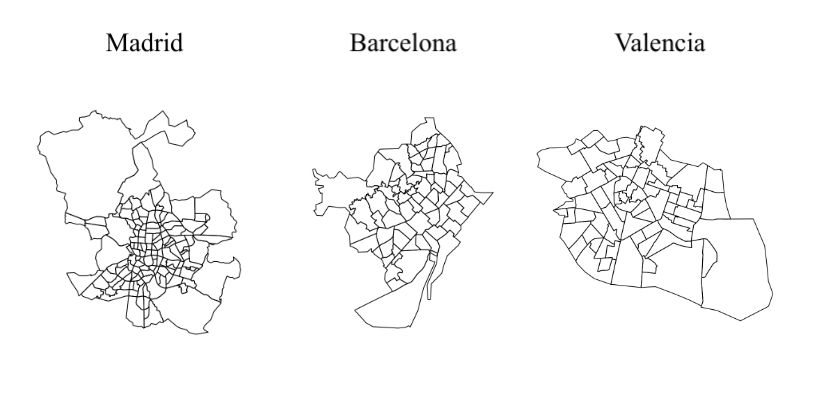
\includegraphics[height=4.5cm]{figures/idealista18-all-polygons}
  \label{fig:all-polygons}
\end{figure}

We have a total of 73 neigborhoods for Barcelona, 135 for Madrid and 73 for Valencia. Each neighborhood has also two additional variables described in the table \ref{table:data-additional-variables}.

\begin{footnotesize}
\begin{longtable}{p{40mm} c p{63mm}}
\caption{Additional variables for each city} \\
\label{table:data-additional-variables} \\
\hline
\hline
% \endhead
% \hline
% \endfoot
& &\\
\textbf{Variable} & \textbf{Mesurement scale} & \textbf{Description}\\
\hline
& &\\
LOCATIONID & nominal & Unique identifier for the neighborhood \\
LOCATIONNAME & nominal & Neighborhood name \\
& &\\
\hline
\end{longtable}
\end{footnotesize}
% \noindent\textbf{Tip:} do not forget to describe any supplementary data files.]

\section*{Experimental Design, Materials and Methods}
% Year of construction is revised as well, given that original year of construction from listings are entered by users in the web site, therefore subject to errors and incomplete (a 40\% missing rate). To remove any issue we assign cadastral construction year from the nearest cadastral parcel whenever value has an outstanding value (date is after publication date or year of construction is before 1500) or when the field value was missing.

The data encompassed three major cities in Spain: Madrid, Barcelona and Valencia, for each municipality we provide listing prices for multi-familiy homes on a quarterly basis. The files contain the complete offering for each of the four quarters in 2018 on idealista web site \cite{idealista}. Idealista is the major real estate listing portal in Spain and also present in other southern european countries as Italy and Portugal.Given the spanish regulatory restrictions idealista listings are slighly anonymized, in order to agree regulatory requirements guaranteeing their attributes and spatial properties. This process take two steps, the first consists of the obfuscation of prices adding or substracting a random percentage of their original values ranging from -2.5\% to +2.5\%. Since asking prices are not normally a completely continuous magnitude (sale prices are usually multiples of 1000 and rent prices are of 10), after the first price modification we finally align prices to multiples of 1000.Finally we carry out a spatial masking process that intends to keep spatial properties of the original data set. As we can see in the figure \ref{fig:points-moved-image} the area where the new point (masked) would be located will be taken randomly within maximum and minimum displacement distances circles. In order to preserve the nature of the neighborhood the house we make sure the new point would fall in the original neighborhood, otherwise we look for a new masked place.

\begin{figure}[!ht]
  \caption{Masking coordinates spatial range. Source: own elaboration}
  \centering
  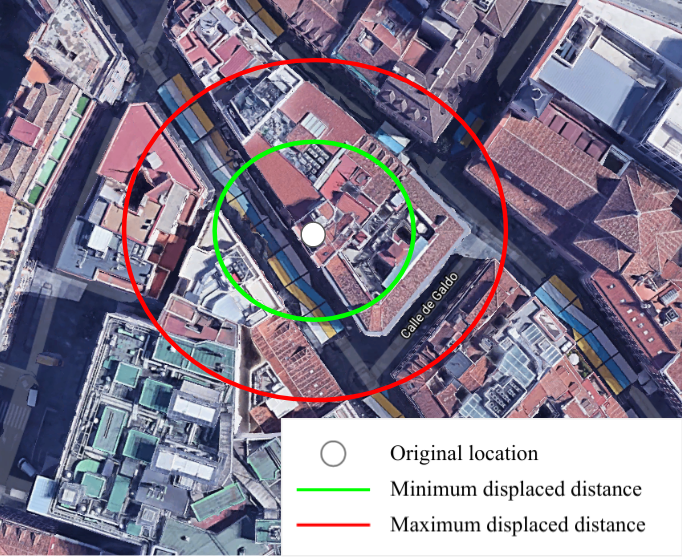
\includegraphics[width=5cm, height=4.3cm]{figures/points-moved-image}
  \label{fig:points-moved-image}
\end{figure}

The algorithm \ref{algo:coordinates-displacement} iteratively  displace the coordinates of each listing with a minimum distance and a maximum distance with the restriction that every new location must fall in within the original neighborbood of the listing.


\begin{algorithm}[!ht]
 \KwData{all idealista listings}
 \KwResult{all idealista listings with masked coordinates}
 initialization\;
 \For{each listing L}{
  take geographical location of L as $(X,Y)$
  \Repeat{this stop condition}{
    take a random angle $\alpha$ from 0 to 360 degrees
    take a distance $R$ as a random value from 30 to 60 meters
    determine a new point $(X',Y')$ calculated as a point located $R$ with the angle $\alpha$
  }
  set $(X',Y')$ as the new location for the listing L
 }
 \caption{Coordinate displacement process for anonymisation purposes}
 \label{algo:coordinates-displacement}
\end{algorithm}

In the figure \ref{fig:coordinates-displacement} we display the histogram with the displacement in meters for all listings in the city of Valencia, as average the displacement is 45 meters.

\begin{figure}[!ht]
  \caption{Coordinate displacement in meters Valencia. Source: own elaboration}
  \centering
  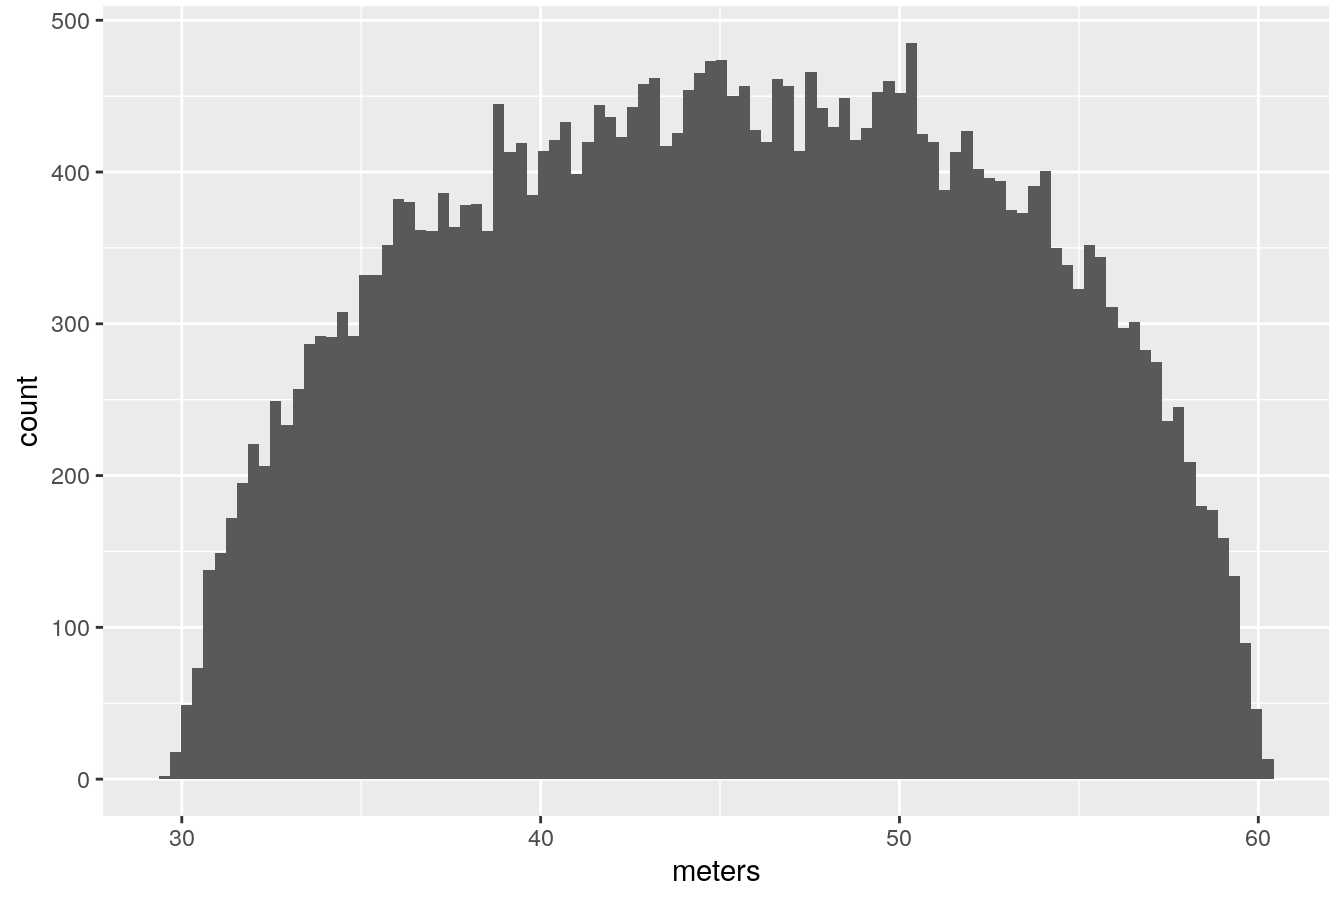
\includegraphics[width=6cm, height=4cm]{figures/coordinates/coordinates-valencia}
  \label{fig:coordinates-displacement}
\end{figure}


% Define a new subcommand
In the figure \ref{fig:points-pre-post-all} we can see the spatial distribution of the original records compared to spatial distribution after masking.

\begin{figure}[!ht]
  \caption{Spatial distribution of ads (before and after masking). Source: own elaboration}
  \centering
  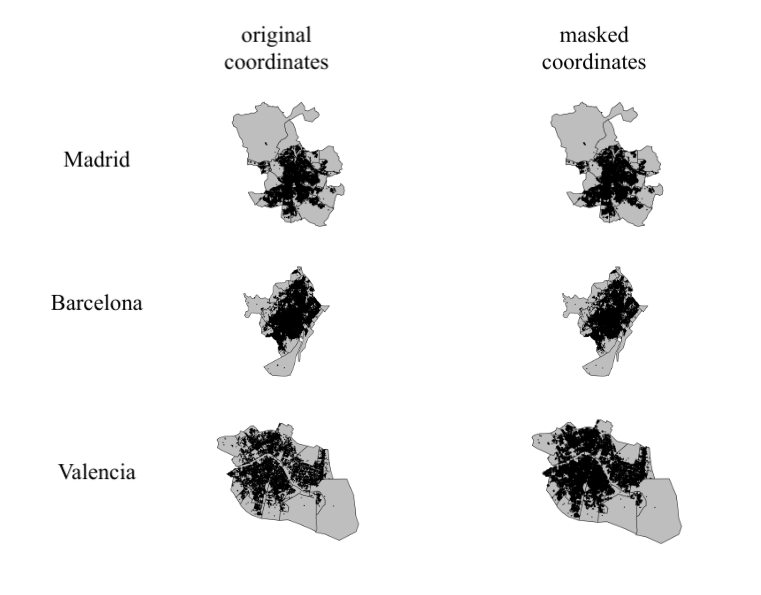
\includegraphics[width=8cm]{figures/points-pre-post-all}
  \label{fig:points-pre-post-all}
\end{figure}



% \noindent [Offer a complete description of the experimental design and methods
% used to acquire these data. Please provide any programs or code files
% used for filtering and analyzing these data. It is very important that
% this section is as comprehensive as possible. If you are submitting via
% another Elsevier journal (a co-submission) you are encouraged to
% provide more detail than in your accompanying research article. There
% is no character limit for this section; however, no insight,
% interpretation, or background should be included in this section.
%
% \noindent\textbf{Tip:} do not describe your data (figures, tables, etc.) in this section,
% do this in the Data Description section above.]

% \section*{Ethics Statement}
% \noindent [Please refer to the journal's
% \href{https://www.elsevier.com/journals/data-in-brief/2352-3409/guide-for-authors}{Guide for Authors}
% for more information on
% the ethical requirements for publication in Data in Brief. In addition
% to these requirements:
%
% \noindent\textbf{If the work involved the use of human subjects:}
% please include a statement here confirming that informed consent was
% obtained for experimentation with human subjects;
%
% \noindent\textbf{If the work involved animal experiments:} please
% include a statement confirming that all experiments comply with
% the \href{https://www.nc3rs.org.uk/arrive-guidelines}{ARRIVE\ guidelines} and were be carried out in accordance with the
% U.K. Animals (Scientific Procedures) Act, 1986 and associated
% guidelines, \href{https://ec.europa.eu/environment/chemicals/lab_animals/legislation_en.htm}{EU Directive 2010/63/EU for animal experiments}, or the
% National Institutes of Health guide for the care and use of Laboratory
% animals (NIH Publications No. 8023, revised 1978)]

\section*{Acknowledgments}

The authors thank Alessandro Galesi for his support in the paper revision and Juan Ramon Selva for collecting and cleaning the spatial data.

% Acknowledgments should be inserted at the end of the paper, before the
% references, not as a footnote to the title. Use the unnumbered
% Acknowledgements Head style for the Acknowledgments heading.

\section*{Declaration of Competing Interest}

The authors declare that they have no known competing financial interests or personal relationships which have, or could be perceived to have, influenced the work reported in this article.

% \noindent [All authors are required to report the following information:
% \begin{enumerate}
% \item[(1)] All third-party financial support for the work this article;
%
% \item[(2)] All financial relationships with any entity that could be
% viewed as relevant to data described in this manuscript;
%
% \item[(3)] All sources of revenue with relevance to this work where
% payments have been made to authors, or their institutions on their
% behalf, within the 36 months prior to submission;
%
% \item[(4)] Any other interactions with the sponsor, outside of the
% submitted work;
%
% \item[(5)] Any relevant patents or copyrights (planned, pending or
% issued);
%
% \item[(6)] Any other relationships or affiliations that may be
% perceived by readers to have influenced, or give the appearance of
% potentially influencing, what has been written in this article.
% \end{enumerate}
% As a general guideline, it is usually better to
% disclose a relationship than not. This information will be acknowledged
% at publication in the manuscript. If there is no known competing
% financial interests or personal relationships that could have appeared
% to influence the work reported in this paper, please include this
% statement.]
%
% \vskip12pt\noindent
% The authors declare that they have no known competing
% financial interests or personal relationships which have, or could be
% perceived to have, influenced the work reported in this article.
%
% \vskip12pt\noindent
% [If there are financial interests/personal relationships which may be
% considered as potential competing interests, please declare them here.]
%
% \subsection*{Note}
% \label{sec1}
% Any instructions relevant to the \verb+elsarticle.cls+ are applicable
% here as well. See the online instruction available on:
% \makeatletter
% \if@twocolumn
% \begin{verbatim}
%  http://support.river-valley.com/wiki/
%  index.php?title=Elsarticle.cls
% \end{verbatim}
% \else
% \begin{verbatim}
%  http://support.river-valley.com/wiki/index.php?title=Elsarticle.cls
% \end{verbatim}
% \fi

% \section*{References}

% \noindent [References are limited (approx. 15) and excessive self-citation is not
% allowed. \textbf{If your data article is co-submitted via another Elsevier
% journal, please cite your associated research article here.}
%
% \noindent\textbf{Reference style:}
% Text:?Indicate references by number(s) in square brackets in line with
% the text. The actual authors can be referred to, but the reference
% number(s) must always be given.?
%
% \noindent Example: '..... as demonstrated [3,6]. Barnaby and Jones [8] obtained a different result ....'?
%
% \noindent [Use \verb+\cite+ command to cite a reference list item in text.
%
% \noindent These are examples for reference citations \cite{1}.
% \cite{2}.
% \cite{4}.]


%% Numbered
%%If
\bibliographystyle{model1-num-names}
\bibliography{refs.bib}



\end{document}

%%
